\documentclass[11pt]{article}
\usepackage{fontspec}
\usepackage{unicode-math}
\setmainfont{TeX Gyre Pagella}
\setmathfont{Latin Modern Math}
\usepackage[margin=1.1in]{geometry}
\usepackage{amsmath}
\usepackage{microtype}
\usepackage{hyperref}
\hypersetup{colorlinks=true,linkcolor=black,citecolor=black,urlcolor=black}
\usepackage{tikz}
\usetikzlibrary{arrows.meta,positioning}
\setlength{\parskip}{0.45em}
\linespread{1.08}

\title{The Rerouted Observable\\[0.3em]
\large Self-Interaction, Scalar Sirens, and the Inverse Probe of Invisible Populations}
\author{Flyxion\\ \small Independent Researcher}
\date{September 2026}

\begin{document}
\maketitle

\begin{abstract}
Gavilan-Martin, Simon, Krishna, Jackson Kimball, Budker, and Wickenbrock propose that rotating black holes surrounded by a self-interacting ultralight scalar can settle into a long-lived state in which angular momentum is continuously carried from the hole to infinity by coherent, nonrelativistic scalar radiation. They call such objects black hole scalar sirens, and they compute the aggregate scalar background expected from the roughly $10^{8}$ isolated stellar-mass black holes in the Milky Way. This essay reads the proposal as an instance of a general structural pattern: an interaction that suppresses the conventional observable of a process reorganizes that process into a different, persistent channel, and the new channel carries information the old one could not. Three levels are kept separate throughout: what the paper computes, what remains physically and observationally unresolved, and what general architecture the result exemplifies. Because the intermediary stores so little of the conserved quantity, the siren also separates persistence of a state from persistence of the regime that regenerates it. A criterion is proposed for when a claim of this kind (``suppression is really rerouting'') is substantive rather than rhetorical: there must be a conserved quantity whose extraction continues, an identified exit channel with a computable flux, and a projection under which that flux is observable.
\end{abstract}

\section{Suppression Under a Projection}

A physical process is almost never observed directly. It is observed through a projection: a detector, a coupling, a frequency band, a statistical estimator. When the projection returns less than expected, the natural inference is that the process has weakened. That inference is valid only if the process has a single exit. If it has several, a reduction in one output may be the signature of increased traffic through another.

The superradiant instability of rotating black holes has, for more than a decade, been studied mainly through two projections. The first is the black hole's spin: if an ultralight boson exists in the right mass range, rapidly rotating holes should have been spun down, so the observation of high-spin holes constrains the boson \cite{ArvanitakiDubovsky2011,ArvanitakiBaryakhtarHuang2015}. The second is gravitational radiation from the bosonic cloud, emitted as a nearly monochromatic signal while the cloud slowly dissipates. Both projections presuppose a particular life history for the cloud: it grows, saturates, and then decays.

The paper under discussion, published in \emph{Physical Review D} on 16 September 2026 \cite{GavilanMartin2026}, starts from the observation that sufficiently strong scalar self-interaction changes that life history. The cloud stays small; its gravitational-wave output drops; the black hole keeps most of its spin. Under the two standard projections the phenomenon looks suppressed. The authors show that it has instead been rerouted: angular momentum still leaves the hole, but it leaves as scalar radiation that escapes to infinity, and it does so steadily over timescales that can exceed the age of the Galaxy.

\section{The Gravitational Atom and Its Standard Life History}

A scalar field of mass $\mu$ around a Kerr black hole of mass $M$ admits quasi-bound states whose spectrum, in the regime of small gravitational fine-structure constant
\begin{equation}
\alpha \equiv \frac{G M \mu}{\hbar c},
\end{equation}
is approximately hydrogenic \cite{Detweiler1980,BaumannChiaPorto2019}. Labelling levels by $n\ell m$ as in hydrogen and working in units $\hbar=c=1$, the leading-order frequencies are
\begin{equation}
\omega_{n\ell m} \simeq \mu\left(1 - \frac{\alpha^{2}}{2n^{2}}\right).
\label{eq:levels}
\end{equation}
A level grows exponentially when its frequency satisfies the superradiance condition $\omega < m\,\Omega_{H}$, where $\Omega_{H}$ is the angular velocity of the horizon \cite{Zeldovich1971,PressTeukolsky1972,BritoCardosoPani2015}. The fastest-growing level is typically $211$. In the absence of self-interaction, the $211$ cloud grows by extracting the hole's rotational energy and angular momentum until $\Omega_{H}$ falls to the threshold, at which point growth stops and the cloud decays, principally through pair annihilation of scalars into gravitons.

This is a depletion architecture. Angular momentum is taken from the hole once, stored in the cloud, and released over the cloud's decay time. The observable traces of the process are the deficit left in the hole's spin and the gravitational signal emitted as the store empties. Once the store is empty, the episode is over.

\section{The Autoionizing Atom}

Scalars with a quartic self-interaction, as for an axion-like field with decay constant $f$ and effective coupling $\lambda \sim \mu^{2}/f^{2}$, can scatter off one another inside the cloud. Baryakhtar, Galanis, Lasenby, and Simon showed that for sufficiently small $f$ the relevant processes drive the $211$ and $322$ levels into a quasi-equilibrium \cite{Baryakhtar2021}. Two scatterings matter most. In the first, two $211$ scalars convert into a $322$ scalar and a scalar absorbed by the hole, populating $322$. In the second,
\begin{equation}
322 + 322 \;\longrightarrow\; 211 + \infty ,
\label{eq:ionize}
\end{equation}
one scalar drops back into the superradiant level while its partner is ejected to infinity. Gavilan-Martin et al.\ describe the resulting configuration as an autoionizing gravitational atom, and it is the second process that turns the cloud into a source.

\begin{figure}[h]
\centering
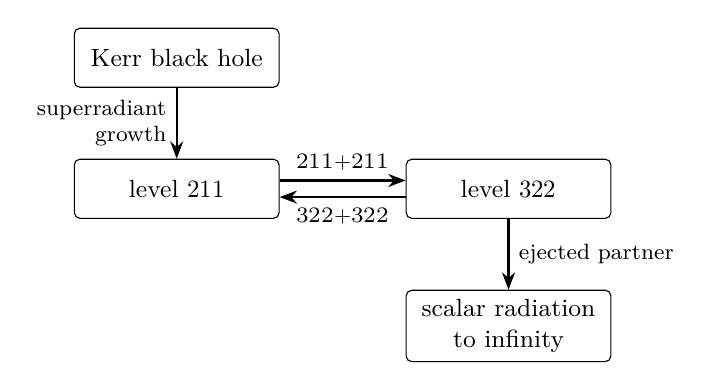
\begin{tikzpicture}[
  node distance=0.9cm and 1.6cm,
  box/.style={draw, rounded corners=2pt, minimum width=2.6cm, minimum height=0.75cm, align=center, font=\small},
  arr/.style={-{Stealth[length=2.2mm]}, thick}
]
\node[box] (bh) {Kerr black hole};
\node[box, below=of bh] (a211) {level $211$};
\node[box, right=of a211] (a322) {level $322$};
\node[box, below=of a322] (inf) {scalar radiation\\to infinity};
\draw[arr] (bh) -- node[left, font=\footnotesize, align=right]{superradiant\\growth} (a211);
\draw[arr] ([yshift=3pt]a211.east) -- node[above, font=\footnotesize]{$211{+}211$} ([yshift=3pt]a322.west);
\draw[arr] ([yshift=-3pt]a322.west) -- node[below, font=\footnotesize]{$322{+}322$} ([yshift=-3pt]a211.east);
\draw[arr] (a322) -- node[right, font=\footnotesize]{ejected partner} (inf);
\end{tikzpicture}
\caption{Schematic flow of angular momentum in the self-interacting regime. The two levels form a bounded intermediary between the hole and infinity.}
\end{figure}

The energetics of \eqref{eq:ionize} fix the velocity of the ejected scalar. Using \eqref{eq:levels} for $n=3$ and $n=2$, conservation of energy gives
\begin{equation}
\omega_{\infty} = 2\omega_{322} - \omega_{211}
\simeq \mu\left(1 + \frac{\alpha^{2}}{8} - \frac{\alpha^{2}}{9}\right)
= \mu\left(1 + \frac{\alpha^{2}}{72}\right).
\end{equation}
The excess over the rest mass is kinetic, $\tfrac12 \mu v^{2} \simeq \mu\alpha^{2}/72$, so that at leading hydrogenic order
\begin{equation}
v \simeq \frac{\alpha}{6} = \frac{G M \mu}{6\,\hbar c}.
\label{eq:velocity}
\end{equation}
At $\alpha \approx 0.2$ this gives $v \approx 0.03c$; extrapolated toward $\alpha \approx 0.5$ it approaches the $\sim 10^{-1}c$ upper end of the velocities quoted by the authors. Either way the emission is far faster than the few $\times 10^{-3}c$ typical of virialized Galactic dark matter. Beyond $\alpha \approx 0.15$ to $0.2$, however, levels other than $211$ and $322$ can become populated (Section~7), and corrections to \eqref{eq:levels} grow, so \eqref{eq:velocity}, which is the paper's own Eq.~(15), should be read as the emission law of the two-level regime rather than a spectrum valid everywhere. Below that threshold the two-level description is not merely an approximation: once equilibrium is reached, the $322$ level suppresses attempts to populate any further level through the same ejection process, so the two-level siren is self-protecting. The scaling is nevertheless the key to everything that follows: at fixed $\mu$, the velocity of the emitted radiation is proportional to the mass of the black hole that emitted it.

\section{Reservoir and Circulator}

The structural change can be stated with a two-variable balance. Let $J_{\rm BH}$ be the hole's angular momentum and $J_{c}$ that of the cloud. Let $\Gamma_{\rm in}$ denote the rate at which superradiance transfers angular momentum into the cloud and $F_{\rm out}$ the rate at which the cloud loses it, whether to gravitons or to escaping scalars. Then
\begin{equation}
\dot J_{c} = \Gamma_{\rm in} - F_{\rm out}, \qquad \dot J_{\rm BH} = -\Gamma_{\rm in}.
\end{equation}

In the depletion architecture, $F_{\rm out}$ is small while the cloud grows, so $J_{c}$ accumulates; growth stops when the hole reaches threshold; the cloud then empties on its decay time. The signal is a single episode whose duration is set by the slowest of these stages.

In the self-interacting regime, $F_{\rm out}$ rises with the occupation of $322$, which rises with that of $211$. The system reaches a state with $\dot J_{c} \approx 0$ while $\Gamma_{\rm in} = F_{\rm out} \neq 0$. The cloud's angular momentum is bounded, yet angular momentum flows through it continuously. The authors describe the equilibrium cloud as an auxiliary that circulates angular momentum from the hole to infinity, and the term is precise: the cloud has stopped being a reservoir and become a conduit.

Two timescales define whether a given hole is a siren. Growth must be fast compared with the age of the Galaxy, $\tau_{\rm grow} \ll t_{\rm gal}$, so that the equilibrium is established. Spin-down must be slow, $\tau_{J} \equiv J_{\rm BH}/F_{\rm out} \gg t_{\rm gal}$, so that the equilibrium persists. The paper's central finding is that there are parameters $(\mu, f)$ for which both hold across a large part of the stellar-mass black hole population. In that window the hole loses only a small fraction of its spin over the Galaxy's lifetime while radiating the whole time.

The circulator has a further property that a reservoir lacks. Because the equilibrium cloud holds only a small fraction of the system's angular momentum, destroying the cloud does not destroy the conditions that produced it. A reservoir that is emptied takes its accumulated store with it; a conduit that is cut leaves the source intact, and the source can open a new conduit. This distinguishes two senses of persistence. State persistence is the continued existence of a particular configuration. Regime persistence is the continued availability of the dynamics that regenerate that configuration. A siren can lose the first and keep the second, and Section~7 shows why this matters physically.

The two architectures can be summarized as
\begin{gather*}
\text{source} \rightarrow \text{accumulation} \rightarrow \text{terminal depletion}\\
\text{versus}\\
\text{source} \rightarrow \text{bounded intermediary} \rightarrow \text{persistent flux}.
\end{gather*}
What distinguishes them is not the total quantity extracted but where the quantity resides at any moment. In the first, the extracted angular momentum is mostly held; in the second, it is mostly in transit.

\section{Persistence Converts Population into Signal}

A single siren is weak and its emission falls off with distance. The observational case rests on aggregation, and aggregation depends on persistence.

Suppose a population of $N$ sources formed at roughly uniform times over the age of the Galaxy, each emitting for a duration $\tau_{\rm emit}$. The fraction emitting at any given moment is approximately $\min(1, \tau_{\rm emit}/t_{\rm gal})$. For transient sources such as mergers, this fraction is tiny, and an observation must catch an individual event in the act. For sirens, with $\tau_{\rm emit} \gtrsim t_{\rm gal}$, the fraction approaches unity. The observer therefore receives contributions from essentially the entire eligible population, each evaluated at its own retarded time. Because the scalars are nonrelativistic, those lookback times exceed $r/c$, but they remain short compared with the age of the population, while the emission lifetime is Galactic. The ensemble is therefore only weakly sensitive to the detailed formation history of the black holes. With $N \sim 10^{8}$ isolated stellar-mass black holes \cite{GavilanMartin2026}, this is the difference between waiting for a coincidence and standing inside a field.

A second feature of steady nonrelativistic emission is worth making explicit. For an isotropic steady source of power $L$ emitting radiation that streams freely at speed $v$, the elementary transport estimate of the energy density at distance $r$ is
\begin{equation}
\rho(r) \sim \frac{L}{4\pi r^{2} v}.
\end{equation}
This is the angle-averaged form of the nonrelativistic flux relation the paper uses to normalize the radiated field, in which total power equals $\mu^{2}\langle\phi^{2}\rangle v$ integrated over a sphere. Siren emission is not isotropic, however: the dominant angular component goes as $\sin^{3}\vartheta$, so emission peaks toward the equatorial plane of each hole, and the paper carries the full radiation pattern through a population integral over the radiated field and its gradient. The $1/v$ factor nevertheless captures a real transport fact. At fixed outward power, slower radiation corresponds to a larger instantaneous energy inventory within a given radial volume. Summing over sources with independent phases, energy densities add, and the local background becomes a weighted integral over the Galactic distribution of holes. Because that distribution is concentrated toward the Galactic Center, so is the flux arriving at Earth, and the arriving field has a net direction. The authors call this directional component a scalar wind. For detectors with a directional axis, such as polarized atomic or nuclear spins coupling to the field gradient, Earth's rotation sweeps that axis through the wind, and depending on the orientation of the rotation plane relative to the Galactic disk, the signal can drop by up to about ninety percent from its maximum over a day. The wind from dark matter blows opposite Earth's motion through the halo; the siren wind blows from the Galactic Center, so the modulation also discriminates between the two. The rerouted observable therefore has not only a magnitude but a temporal signature. The resulting local energy density is small, below about $10^{-5}\,\mathrm{GeV/cm^{3}}$ at the Sun against roughly $0.4\,\mathrm{GeV/cm^{3}}$ for halo dark matter, but the higher velocities compensate in the wind observable. The paper reports wind signals up to two orders of magnitude larger than those expected from a pre-inflationary misaligned scalar with the same mass and decay constant, and it emphasizes that the target does not depend on early-universe production or initial conditions \cite{GavilanMartin2026}.

That independence deserves emphasis. Most searches for ultralight scalars assume the field constitutes some or all of the dark matter, which requires a cosmological production story. A siren background requires only that the field exist with suitable $\mu$ and $f$ and that the Galaxy contain spinning black holes. The source of the signal is present-day astrophysics.

\section{The Inverse Channel}

The aggregate field is not an undifferentiated hum. Its structure can be decomposed along the lines of what each part of the emission process encodes.

The carrier scale fixes the scalar mass to leading order. Every emitted quantum oscillates at $\omega_{\infty} \simeq \mu(1 + v^{2}/2)$, slightly above $\mu$ because of the kinetic energy of the escaping scalar. Source and observer motion add Doppler structure, but it is subdominant: both the black holes and Earth move below the Galactic escape velocity, while the emitted scalars must exceed it to reach us at all. The low-frequency edge of the band therefore determines $\mu$, while its width and shape carry information about the emitting population.

The structure within that band encodes black hole masses. By \eqref{eq:velocity}, each hole contributes at a velocity proportional to its mass. Once $\mu$ is known from the carrier, the velocity distribution of the background is, to leading order, a rescaled image of the mass distribution of the emitting population, weighted by each source's power and distance. The authors state the corresponding result directly: at fixed scalar mass, the spectral shape is set primarily by the black hole mass distribution.

Spin enters differently. A hole is a siren only if it rotates fast enough to satisfy the superradiance condition for $211$ at the relevant $\alpha$. Spin therefore acts less as a coordinate on the spectrum than as a gate on participation: it determines which holes contribute, and so it shows up mainly in the amplitude of the signal, which the authors find sensitive to the spin-distribution parameter, rather than in its shape.

Direction and modulation encode spatial distribution. The concentration toward the Galactic Center and the daily modulation carry information about where the emitting population lies.

Put together, the observational architecture runs backwards from the usual order of astronomy:
\begin{gather*}
\text{invisible population} \rightarrow \text{scalar emission}\\
\rightarrow \text{spectral and directional structure} \rightarrow \text{inference about the population}.
\end{gather*}
Isolated stellar-mass black holes are among the hardest objects in the Galaxy to observe. They are not accreting, not merging, and not in binaries whose companions betray them; apart from rare microlensing events they emit essentially nothing through conventional channels. The siren proposal makes them collectively luminous in a channel that, if it exists, is sensitive precisely to the property that makes them otherwise dark: they are alone, spinning, and undisturbed. The authors stress the possibility of joint discovery. A detection would establish a new field and, in the same measurement, deliver a census of a population that has so far been counted only through stellar-evolution models.

The inverse problem is not trivially invertible, and the paper is specific about where it strains. The mass-to-velocity correspondence requires that the distance and mass distributions of the holes be independent, so that distance factors out as an overall amplitude. The spin gate couples to the mass mapping because the superradiance threshold tightens as $\alpha$ grows. For populations with characteristic $\alpha$ above about $0.15$, individual sirens may emit polychromatically; their rest-frame spectra then act as a convolution kernel on the ensemble line and blur its relation to the mass function. And because the true mass function is known only through models, a search tuned to a detailed lineshape risks overfitting, which is why the authors treat a broadband template as the conservative strategy. After a detection, the direction reverses: accurate modeling of the rest-frame spectrum would allow deconvolution to separate intrinsic siren structure from the mass distribution. A realistic analysis would be a hierarchical inference over population parameters, of the kind used for gravitational-wave population studies, rather than a direct reading. The claim is not that the spectrum is a photograph of the population, but that it is a projection that preserves population structure a null background would erase.

\section{What Is Established and What Is Not}

The paper is theoretical, and four qualifications bound what it establishes. They are worth separating.

First, the field must exist, with a mass placing $\alpha$ in the superradiant range for stellar-mass holes and a decay constant $f$ in the window where both timescale conditions hold: for stellar-mass sirens, masses of roughly $10^{-13}$ to $10^{-11}$\,eV and $f$ below about $10^{14}$ to $10^{9}$\,GeV across that range. Nothing in current data requires such a field.

Second, the quasi-equilibrium description has a controlled domain. At sufficiently small $\alpha$, the $211$ and $322$ levels dominate and the two-level siren of Baryakhtar et al.\ \cite{Baryakhtar2021} is the relevant description. As $\alpha$ increases beyond roughly $0.15$ to $0.2$, additional hydrogenic levels can acquire appreciable occupation and the emitted spectrum may become polychromatic. A finite multilevel quasi-equilibrium is plausible, but a systematic convergent treatment of that regime has not been developed, and the authors restrict their principal analysis to $\alpha < 0.5$.

Third, environmental perturbations can interrupt a siren without necessarily destroying its capacity to recur. A companion can mix levels, ionize the cloud, or preferentially strip the more extended $322$ level and so break the quasi-equilibrium \cite{BaumannChiaPorto2019,Takahashi2024}. Yet the equilibrium cloud holds only a small fraction of the system's angular momentum. If a transient perturbation removes the cloud without substantially altering the black hole, superradiant growth can rebuild it once the perturbation has passed, and the authors describe exactly this rebirth of the siren. A sustained perturbation is more complicated. In an inspiral, stripping the $322$ level can let the $211$ level resume growth until attractive self-interactions collapse the cloud, and the siren may enter a repeater phase of growth and collapse before continuous emission resumes; whether such cycles extract angular momentum efficiently is left open. Few stellar-mass black holes have companions at all, only a few percent by the estimates the paper cites, so the authors fold this uncertainty into the count of emitting holes, and they note that any gradual degradation of sirens would show up as a spin distribution tilted toward low spin, itself a signature of superradiance. This is the regime persistence of Section~4 in physical form: what persists is not the uninterrupted identity of a particular cloud but the dynamical capacity to regenerate the emitting state. It is also why the argument depends so directly on the circulator structure. A reservoir stripped of its store would have to repeat the entire extraction; a circulator stripped of its conduit only has to reopen it. The number, mass function, spin distribution, and spatial distribution of the target population nonetheless remain model-dependent, and the predicted signal inherits those uncertainties.

Fourth, detection requires instruments sensitive to a coherent field at the relevant frequency, with enough resolution to see the broadened spectrum and, for the directional signal, a directional axis such as polarized spins. The authors note that haloscope-style experiments can in principle search for this nonprimordial population. Detection also requires a coupling between the scalar and ordinary matter, which is a separate parameter from anything in the siren physics. The authors' benchmark wind signal at Earth is of order $10^{-27}$\,eV, while current nuclear-spin techniques reach energy resolutions around $10^{-25}$\,eV, leaving a gap of two to three orders of magnitude. Recasting existing dark-matter limits reaches only couplings far larger than effective field theory would naturally suggest. The paper therefore presents sirens as a well-defined target for next-generation spin-based and magnetic searches, not as something current data can test.

One consequence holds regardless of detection. The exclusions drawn from the conventional channels are conditional on the self-interaction regime. Parameter space disfavored by black hole spin measurements under negligible self-interaction can reopen when strong self-interaction drives the cloud into the siren regime; the scalar mass range of interest overlaps a range that high-spin observations would otherwise disfavor. Gravitational-wave searches and scalar-emission searches, meanwhile, probe complementary and effectively exclusive dynamical regimes: negligible self-interaction favors gravitational emission, strong self-interaction favors scalar radiation. A null result in one channel constrains its own regime and says little about the other.

\section{When Suppression Is Rerouting}

The general reading of the paper is easy to state and easy to abuse. Stated plainly: an interaction that reduces the observable output of a process may be reorganizing that process into a different persistent channel rather than weakening it. Abused, this becomes a way of never accepting a null result, since any absence can be redescribed as displacement into some unobserved channel.

The siren case shows what separates the substantive version from the rhetorical one. Three conditions hold.

A conserved quantity continues to flow. Angular momentum leaves the black hole in both regimes. Because it is conserved, a decrease in one output with continued extraction obliges an increase somewhere else. The claim of rerouting is backed by bookkeeping, not by a preference for continuity.

The exit channel is identified and its flux is computable. The process \eqref{eq:ionize} is a specific scattering with calculable rate and kinematics. The claim is not that the missing output has gone somewhere, but that it has gone to a named place at a predicted rate with a predicted velocity.

The exit is observable under some projection. The rerouted flux has a carrier frequency, a spectrum, a direction, and a modulation. It can therefore fail. The authors state the falsification condition themselves: given strong priors on the scalar's coupling to ordinary matter, a confident failure to observe the stellar-mass siren background would exclude the minimal parameter space with $f < f_{\rm siren}$ in this mass range, up to uncertainties in the black hole population, and it would do so in exactly the region where the conventional channels had gone quiet. The qualification matters. The projection $\Pi_b$ has its own free parameter, the coupling through which the detector sees the field, and a null result constrains the rerouting claim only jointly with a claim about that coupling. The criterion keeps its force, but it shows that ``observable under some projection'' is itself a hypothesis to be stated, not a given.

Written as bookkeeping, with $Q$ the conserved quantity, $F_{\rm source}$ the rate at which it leaves the source, $F_a$ and $F_b$ the fluxes through the original and alternative channels, and $\Pi_b$ the projection that observes channel $b$, the criterion reads
\begin{equation}
\left.
\begin{aligned}
&\dot Q_{\rm store} \simeq 0,\\
&F_{\rm source} > 0,\\
&F_a \downarrow, \quad F_b > 0,\\
&\Pi_b(F_b) \neq 0
\end{aligned}
\;\right\}
\;\Longrightarrow\;\; \text{dynamically identifiable rerouting}.
\end{equation}
The first two conditions say the intermediary is not accumulating while extraction continues, so the extracted quantity must be leaving. The third says it is leaving by a different route. The fourth says the new route can be seen. Suppression alone, $F_a \downarrow$, implies none of this.

When all of these hold, suppression under one projection is correctly described as a transition to another dynamical channel. When the first fails, there is no obligation that anything went anywhere. When the second fails, the claim is unfalsifiable. When the third fails, it may be true but cannot be tested. The pattern is common well beyond astrophysics: in chemistry, where an inhibitor redirects a reaction toward a side product; in ecology, where predation pressure shifts energy flow to another trophic path; in institutions, where suppressing one outlet for a pressure reliably relocates the pressure. In each case the same three questions separate insight from evasion: what is conserved, where does it go, and how would one see it arrive.

\section{Conclusion}

The black hole scalar siren is a small cloud doing a large job. By settling into a quasi-equilibrium between two levels, it stops accumulating the black hole's angular momentum and starts transmitting it, so that a feature which made the conventional signals fade also makes the phenomenon last as long as the Galaxy. Because the cloud stores so little, even its destruction is not final: the regime that produced it can produce it again. That longevity converts a population of objects individually too faint to matter into a collective field, and the kinematics of the emission preserve, in the spread of velocities and the direction of arrival, information about the population that produced it.

The broader lesson is about projections. An observable is always a choice of where to look for the output of a process. When an interaction closes the place one was looking, the productive question is whether the process still has something to discharge and where the discharge now goes. Here the answer is specific enough to be computed and definite enough to be refuted, and that is what makes the rerouting a result rather than a consolation.

\begin{thebibliography}{99}

\bibitem{GavilanMartin2026}
D.~Gavilan-Martin, O.~Simon, D.~Krishna, D.~F.~Jackson Kimball, D.~Budker, and A.~Wickenbrock,
``Black hole scalar sirens in the Milky Way,''
\emph{Phys.\ Rev.\ D} \textbf{114}, 055028 (2026); arXiv:2602.23415.

\bibitem{Baryakhtar2021}
M.~Baryakhtar, M.~Galanis, R.~Lasenby, and O.~Simon,
``Black hole superradiance in the presence of axion self-interactions,''
\emph{Phys.\ Rev.\ D} \textbf{103}, 095019 (2021).

\bibitem{ArvanitakiDubovsky2011}
A.~Arvanitaki and S.~Dubovsky,
``Exploring the string axiverse with precision black hole physics,''
\emph{Phys.\ Rev.\ D} \textbf{83}, 044026 (2011).

\bibitem{ArvanitakiBaryakhtarHuang2015}
A.~Arvanitaki, M.~Baryakhtar, and X.~Huang,
``Discovering the QCD axion with black holes,''
\emph{Phys.\ Rev.\ D} \textbf{91}, 084011 (2015).

\bibitem{Detweiler1980}
S.~Detweiler,
``Klein-Gordon equation and rotating black holes,''
\emph{Phys.\ Rev.\ D} \textbf{22}, 2323 (1980).

\bibitem{Zeldovich1971}
Ya.~B.~Zel'dovich,
``Generation of waves by a rotating body,''
\emph{JETP Lett.} \textbf{14}, 180 (1971).

\bibitem{PressTeukolsky1972}
W.~H.~Press and S.~A.~Teukolsky,
``Floating orbits, superradiant scattering and the black-hole bomb,''
\emph{Nature} \textbf{238}, 211 (1972).

\bibitem{BritoCardosoPani2015}
R.~Brito, V.~Cardoso, and P.~Pani,
\emph{Superradiance}, Lecture Notes in Physics \textbf{906} (Springer, 2015).

\bibitem{BaumannChiaPorto2019}
D.~Baumann, H.~S.~Chia, and R.~A.~Porto,
``Probing ultralight bosons with binary black holes,''
\emph{Phys.\ Rev.\ D} \textbf{99}, 044001 (2019).

\bibitem{Takahashi2024}
T.~Takahashi, H.~Omiya, and T.~Tanaka,
\emph{Phys.\ Rev.\ D} \textbf{110}, 104038 (2024).

\end{thebibliography}

\end{document}
